% Chapter 6: Transport Layers
\chapter{Transport Layers}
\label{ch:transport-layers}

Transport layers define how \tprotocol{} messages are encoded and transmitted across different communication protocols. The protocol is designed to be transport-agnostic, allowing the same payment logic to work across HTTP, MCP, A2A, and custom transports.

\section{Transport Architecture}
\label{sec:transport-architecture}

\begin{figure}[ht]
\centering
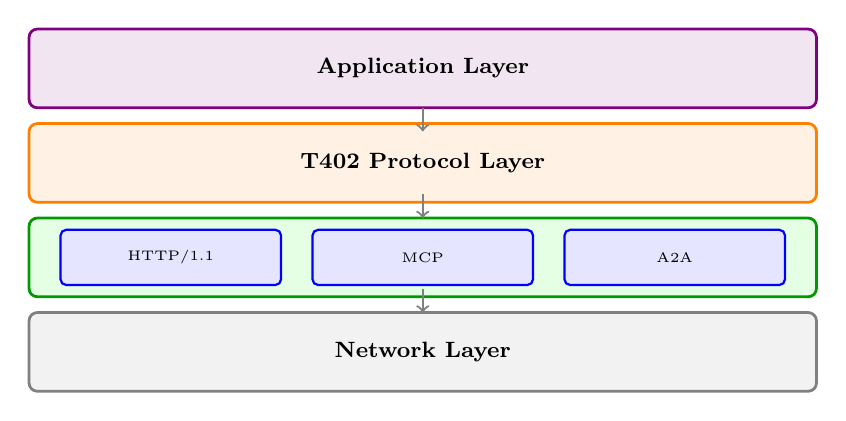
\begin{tikzpicture}[
    layer/.style={
        rectangle,
        rounded corners=3pt,
        minimum width=10cm,
        minimum height=1cm,
        draw=violet,
        line width=1pt,
        fill=violet!10,
        font=\footnotesize\bfseries
    },
    component/.style={
        rectangle,
        rounded corners=2pt,
        minimum width=2.8cm,
        minimum height=0.7cm,
        draw=blue,
        line width=0.8pt,
        fill=blue!10,
        font=\tiny
    }
]

% Layers
\node[layer] (app) at (0,3) {Application Layer};
\node[layer, fill=orange!10, draw=orange] (t402) at (0,1.8) {T402 Protocol Layer};
\node[layer, fill=green!10, draw=green!60!black] (transport) at (0,0.6) {Transport Layer};
\node[layer, fill=gray!10, draw=gray] (network) at (0,-0.6) {Network Layer};

% Transport components
\node[component] at (-3.2,0.6) {HTTP/1.1};
\node[component] at (0,0.6) {MCP};
\node[component] at (3.2,0.6) {A2A};

% Arrows
\draw[->, thick, gray] (0,2.5) -- (0,2.2);
\draw[->, thick, gray] (0,1.4) -- (0,1.1);
\draw[->, thick, gray] (0,0.2) -- (0,-0.1);

\end{tikzpicture}
\caption{Transport layer architecture}
\label{fig:transport-architecture}
\end{figure}

Each transport must implement three core operations:

\begin{table}[ht]
\centering
\caption{Transport Operations}
\label{tab:transport-operations}
\begin{tabular}{l l p{6cm}}
\toprule
\textbf{Operation} & \textbf{Direction} & \textbf{Description} \\
\midrule
Signal Payment & Server $\to$ Client & Transmit PaymentRequirements \\
Receive Payment & Client $\to$ Server & Accept PaymentPayload \\
Return Result & Server $\to$ Client & Send SettlementResponse \\
\bottomrule
\end{tabular}
\end{table}

\section{HTTP Transport}
\label{sec:http-transport}

The HTTP transport is the canonical implementation, using standard HTTP mechanisms for maximum compatibility with existing infrastructure.

\subsection{Header Specification}

\tprotocol{} defines three custom HTTP headers:

\begin{table}[ht]
\centering
\caption{HTTP Headers for T402}
\label{tab:http-headers-detail}
\begin{tabular}{l l p{5.5cm}}
\toprule
\textbf{Header} & \textbf{Direction} & \textbf{Content} \\
\midrule
\header{PAYMENT-REQUIRED} & S $\to$ C & Base64url(PaymentRequirements) \\
\header{PAYMENT-SIGNATURE} & C $\to$ S & Base64url(PaymentPayload) \\
\header{PAYMENT-RESPONSE} & S $\to$ C & Base64url(SettlementResponse) \\
\bottomrule
\end{tabular}
\end{table}

\begin{infobox}[Base64url Encoding]
All header values use Base64url encoding (RFC 4648 \S5) without padding. This ensures compatibility with HTTP header character restrictions and avoids issues with \code{+}, \code{/}, and \code{=} characters.
\end{infobox}

\subsection{Status Code Mapping}

\begin{table}[ht]
\centering
\caption{HTTP Status Code Mapping}
\label{tab:status-codes}
\begin{tabular}{l l l p{4cm}}
\toprule
\textbf{T402 State} & \textbf{HTTP} & \textbf{Header} & \textbf{Body} \\
\midrule
Payment Required & 402 & PAYMENT-REQUIRED & Error JSON \\
Invalid Payload & 400 & -- & Error details \\
Verification Failed & 402 & PAYMENT-RESPONSE & Error details \\
Settlement Failed & 402 & PAYMENT-RESPONSE & Error details \\
Success & 200 & PAYMENT-RESPONSE & Resource \\
Server Error & 500 & -- & Error details \\
\bottomrule
\end{tabular}
\end{table}

\subsection{Request Flow}

\begin{figure}[ht]
\centering
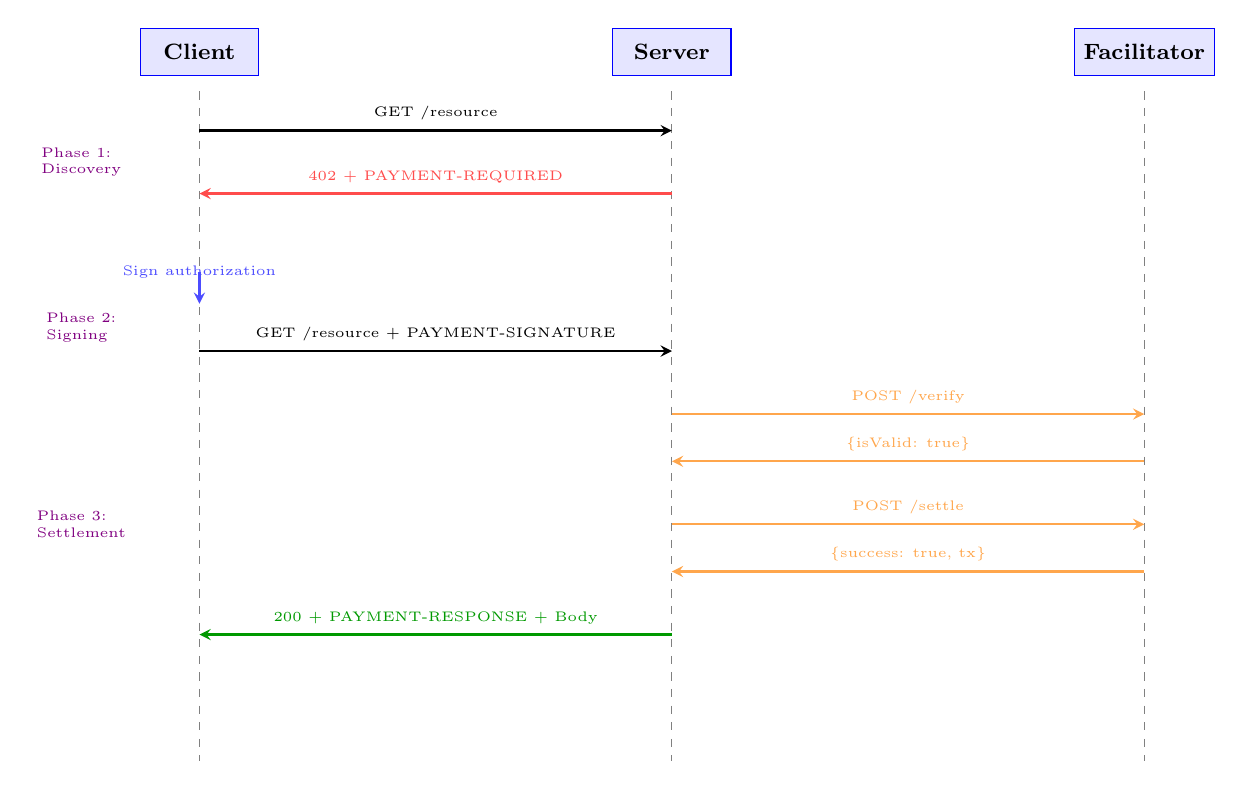
\begin{tikzpicture}[
    actor/.style={
        rectangle,
        minimum width=1.5cm,
        minimum height=0.6cm,
        draw=blue,
        fill=blue!10,
        font=\footnotesize\bfseries
    },
    msg/.style={
        ->,
        >=stealth,
        thick
    },
    note/.style={
        font=\tiny,
        align=left
    }
]

% Actors
\node[actor] (client) at (0,0) {Client};
\node[actor] (server) at (6,0) {Server};
\node[actor] (facilitator) at (12,0) {Facilitator};

% Lifelines
\draw[dashed, gray] (0,-0.5) -- (0,-9);
\draw[dashed, gray] (6,-0.5) -- (6,-9);
\draw[dashed, gray] (12,-0.5) -- (12,-9);

% Messages
\draw[msg] (0,-1) -- node[above, font=\tiny] {GET /resource} (6,-1);
\draw[msg, red!70] (6,-1.8) -- node[above, font=\tiny] {402 + PAYMENT-REQUIRED} (0,-1.8);

\draw[msg, blue!70] (0,-2.8) -- node[above, font=\tiny] {Sign authorization} (0,-3.2);

\draw[msg] (0,-3.8) -- node[above, font=\tiny] {GET /resource + PAYMENT-SIGNATURE} (6,-3.8);

\draw[msg, orange!70] (6,-4.6) -- node[above, font=\tiny] {POST /verify} (12,-4.6);
\draw[msg, orange!70] (12,-5.2) -- node[above, font=\tiny] {\{isValid: true\}} (6,-5.2);

\draw[msg, orange!70] (6,-6) -- node[above, font=\tiny] {POST /settle} (12,-6);
\draw[msg, orange!70] (12,-6.6) -- node[above, font=\tiny] {\{success: true, tx\}} (6,-6.6);

\draw[msg, green!60!black] (6,-7.4) -- node[above, font=\tiny] {200 + PAYMENT-RESPONSE + Body} (0,-7.4);

% Phase labels
\node[note, violet] at (-1.5,-1.4) {Phase 1:\\Discovery};
\node[note, violet] at (-1.5,-3.5) {Phase 2:\\Signing};
\node[note, violet] at (-1.5,-6) {Phase 3:\\Settlement};

\end{tikzpicture}
\caption{HTTP transport message flow}
\label{fig:http-flow}
\end{figure}

\subsection{Complete Example}

\begin{lstlisting}[caption={Phase 1: Initial request and 402 response}]
# Client sends initial request
GET /api/premium/data HTTP/1.1
Host: api.example.com
Accept: application/json
User-Agent: T402-Client/2.0

# Server responds with payment requirements
HTTP/1.1 402 Payment Required
Content-Type: application/json
PAYMENT-REQUIRED: eyJ0NDAyVmVyc2lvbiI6Miwic...
X-T402-Version: 2

{
  "error": "Payment required",
  "code": "payment_required",
  "resource": "/api/premium/data"
}
\end{lstlisting}

\begin{lstlisting}[caption={Phase 2: Request with payment}]
# Client sends request with signed payment
GET /api/premium/data HTTP/1.1
Host: api.example.com
Accept: application/json
PAYMENT-SIGNATURE: eyJ0NDAyVmVyc2lvbiI6Miwi...

# Server returns resource with settlement confirmation
HTTP/1.1 200 OK
Content-Type: application/json
PAYMENT-RESPONSE: eyJzdWNjZXNzIjp0cnVlLC...
X-T402-Transaction: 0x7a8b9c...

{
  "data": { ... }
}
\end{lstlisting}

\subsection{Error Responses}

\begin{lstlisting}[language=json,caption={Payment verification failed}]
HTTP/1.1 402 Payment Required
Content-Type: application/json
PAYMENT-RESPONSE: eyJzdWNjZXNzIjpmYWxzZS...

{
  "error": "Payment verification failed",
  "code": "invalid_signature",
  "details": "Signature does not match payer address"
}
\end{lstlisting}

\begin{lstlisting}[language=json,caption={Insufficient funds}]
HTTP/1.1 402 Payment Required
Content-Type: application/json
PAYMENT-RESPONSE: eyJzdWNjZXNzIjpmYWxzZS...

{
  "error": "Payment failed",
  "code": "insufficient_funds",
  "details": "Payer balance: 0.50 USDT, required: 1.00 USDT"
}
\end{lstlisting}

\subsection{Content Negotiation}

Servers MAY support content negotiation for payment requirements:

\begin{lstlisting}[caption={Content negotiation headers}]
# Client indicates preferred networks
GET /api/data HTTP/1.1
Accept-Payment: network=eip155:8453, network=eip155:42161

# Server responds with filtered options
HTTP/1.1 402 Payment Required
PAYMENT-REQUIRED: eyJ0NDAyVmVyc2lvbiI6Mi...
Vary: Accept-Payment
\end{lstlisting}

\subsection{Caching Considerations}

Payment-protected resources require careful cache handling:

\begin{table}[ht]
\centering
\caption{Cache-Control Directives}
\label{tab:cache-control}
\begin{tabular}{l p{7cm}}
\toprule
\textbf{Response} & \textbf{Recommended Headers} \\
\midrule
402 Response & \code{Cache-Control: no-store} \\
200 with Payment & \code{Cache-Control: private, no-cache} \\
Idempotent Resource & \code{Cache-Control: private, max-age=N} \\
\bottomrule
\end{tabular}
\end{table}

\section{MCP Transport}
\label{sec:mcp-transport}

The Model Context Protocol (MCP) transport enables AI agents to make payments when invoking tools. MCP uses JSON-RPC 2.0 over stdio or HTTP.

\subsection{Architecture Overview}

\begin{figure}[ht]
\centering
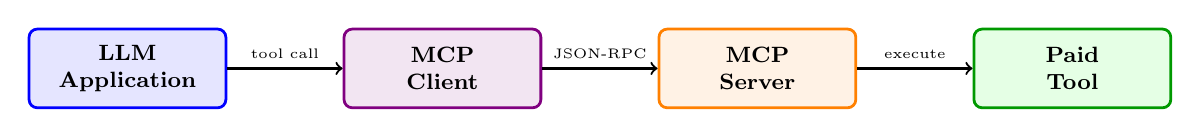
\begin{tikzpicture}[
    box/.style={
        rectangle,
        rounded corners=3pt,
        minimum width=2.5cm,
        minimum height=1cm,
        draw=blue,
        line width=1pt,
        fill=blue!10,
        font=\footnotesize\bfseries,
        align=center
    }
]

\node[box] (llm) at (0,0) {LLM\\Application};
\node[box, draw=violet, fill=violet!10] (client) at (4,0) {MCP\\Client};
\node[box, draw=orange, fill=orange!10] (server) at (8,0) {MCP\\Server};
\node[box, draw=green!60!black, fill=green!10] (tool) at (12,0) {Paid\\Tool};

\draw[->, thick] (llm) -- node[above, font=\tiny] {tool call} (client);
\draw[->, thick] (client) -- node[above, font=\tiny] {JSON-RPC} (server);
\draw[->, thick] (server) -- node[above, font=\tiny] {execute} (tool);

\end{tikzpicture}
\caption{MCP transport architecture}
\label{fig:mcp-architecture}
\end{figure}

\subsection{Tool Discovery}

Paid tools advertise payment requirements in their schema:

\begin{lstlisting}[language=json,caption={MCP tool with payment requirements}]
{
  "jsonrpc": "2.0",
  "id": 1,
  "result": {
    "tools": [{
      "name": "financial_analysis",
      "description": "Analyze stock performance",
      "inputSchema": {
        "type": "object",
        "properties": {
          "ticker": { "type": "string" }
        }
      },
      "t402": {
        "price": "0.05",
        "asset": "USDT",
        "description": "Per-analysis fee"
      }
    }]
  }
}
\end{lstlisting}

\subsection{Payment Required Response}

When a tool requires payment, the server returns a JSON-RPC error:

\begin{lstlisting}[language=json,caption={MCP payment required error}]
{
  "jsonrpc": "2.0",
  "id": 1,
  "error": {
    "code": -32402,
    "message": "Payment required",
    "data": {
      "t402Version": 2,
      "resource": {
        "url": "mcp://server/tools/financial_analysis",
        "method": "tools/call"
      },
      "description": "Financial analysis tool",
      "mimeType": "application/json",
      "accepts": [{
        "scheme": "exact",
        "network": "eip155:8453",
        "asset": "0x833589fCD6...USDC",
        "amount": "50000",
        "payTo": "0xMerchant...",
        "maxTimeoutSeconds": 300
      }]
    }
  }
}
\end{lstlisting}

\subsection{Payment Transmission}

Payments are included in the request's \code{\_meta} field:

\begin{lstlisting}[language=json,caption={MCP tool call with payment}]
{
  "jsonrpc": "2.0",
  "id": 2,
  "method": "tools/call",
  "params": {
    "name": "financial_analysis",
    "arguments": {
      "ticker": "AAPL",
      "period": "1Y"
    },
    "_meta": {
      "t402/payment": {
        "t402Version": 2,
        "accepted": {
          "scheme": "exact",
          "network": "eip155:8453",
          "asset": "0x833589fCD6...USDC",
          "amount": "50000",
          "payTo": "0xMerchant..."
        },
        "payload": {
          "from": "0xPayer...",
          "validAfter": 1704067200,
          "validBefore": 1704070800,
          "nonce": "0x7f8a9b...",
          "signature": "0x2d6a75..."
        }
      }
    }
  }
}
\end{lstlisting}

\subsection{Success Response}

\begin{lstlisting}[language=json,caption={MCP successful response with settlement}]
{
  "jsonrpc": "2.0",
  "id": 2,
  "result": {
    "content": [{
      "type": "text",
      "text": "Analysis for AAPL: ..."
    }],
    "_meta": {
      "t402/settlement": {
        "success": true,
        "network": "eip155:8453",
        "transaction": "0x7a8b9c...",
        "payer": "0xPayer...",
        "amount": "50000"
      }
    }
  }
}
\end{lstlisting}

\subsection{Error Codes}

\begin{table}[ht]
\centering
\caption{MCP T402 Error Codes}
\label{tab:mcp-errors}
\begin{tabular}{l l p{5cm}}
\toprule
\textbf{Code} & \textbf{Meaning} & \textbf{Description} \\
\midrule
-32402 & Payment Required & Tool requires payment \\
-32403 & Payment Failed & Verification or settlement failed \\
-32404 & Invalid Payment & Malformed payment payload \\
-32405 & Expired Payment & Authorization has expired \\
\bottomrule
\end{tabular}
\end{table}

\section{A2A Transport}
\label{sec:a2a-transport}

The Agent-to-Agent (A2A) transport enables direct payments between autonomous AI agents using Google's A2A protocol.

\subsection{A2A Protocol Overview}

A2A defines agent communication primitives:

\begin{itemize}
    \item \textbf{Agent Card}: Discovery and capability advertisement
    \item \textbf{Tasks}: Work requests with structured inputs/outputs
    \item \textbf{Messages}: Communication within task context
    \item \textbf{Artifacts}: Deliverables produced by agents
\end{itemize}

\subsection{Payment in Agent Cards}

Agents advertise payment requirements in their Agent Card:

\begin{lstlisting}[language=json,caption={A2A Agent Card with T402 payment}]
{
  "name": "DataAnalysisAgent",
  "description": "Performs statistical analysis",
  "url": "https://agent.example.com",
  "capabilities": {
    "streaming": false,
    "pushNotifications": false
  },
  "skills": [{
    "id": "regression_analysis",
    "name": "Regression Analysis",
    "inputModes": ["application/json"],
    "outputModes": ["application/json"]
  }],
  "extensions": {
    "t402": {
      "version": 2,
      "paymentEndpoint": "/t402/payment",
      "pricing": {
        "regression_analysis": {
          "amount": "100000",
          "asset": "USDT",
          "network": "eip155:8453"
        }
      }
    }
  }
}
\end{lstlisting}

\subsection{Task Payment Flow}

\begin{figure}[ht]
\centering
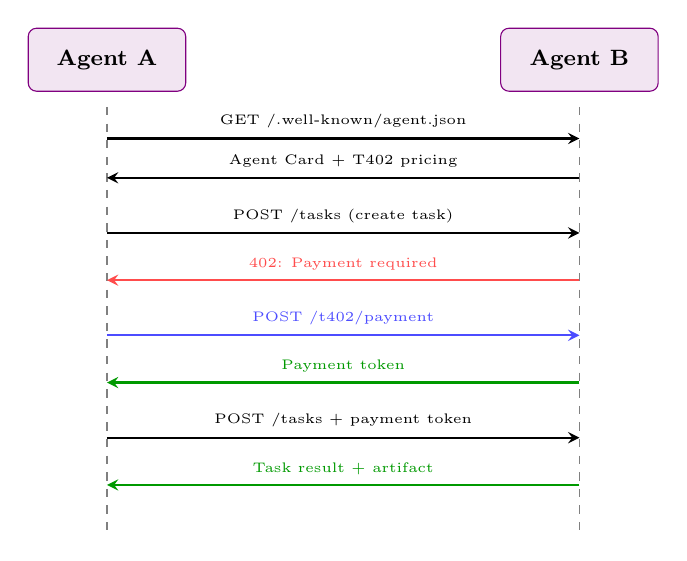
\begin{tikzpicture}[
    agent/.style={
        rectangle,
        rounded corners=3pt,
        minimum width=2cm,
        minimum height=0.8cm,
        draw=violet,
        fill=violet!10,
        font=\footnotesize\bfseries
    },
    msg/.style={->, >=stealth, thick}
]

\node[agent] (a1) at (0,0) {Agent A};
\node[agent] (a2) at (6,0) {Agent B};

\draw[dashed, gray] (0,-0.6) -- (0,-6);
\draw[dashed, gray] (6,-0.6) -- (6,-6);

% Discovery
\draw[msg] (0,-1) -- node[above, font=\tiny] {GET /.well-known/agent.json} (6,-1);
\draw[msg] (6,-1.5) -- node[above, font=\tiny] {Agent Card + T402 pricing} (0,-1.5);

% Task creation
\draw[msg] (0,-2.2) -- node[above, font=\tiny] {POST /tasks (create task)} (6,-2.2);
\draw[msg, red!70] (6,-2.8) -- node[above, font=\tiny] {402: Payment required} (0,-2.8);

% Payment
\draw[msg, blue!70] (0,-3.5) -- node[above, font=\tiny] {POST /t402/payment} (6,-3.5);
\draw[msg, green!60!black] (6,-4.1) -- node[above, font=\tiny] {Payment token} (0,-4.1);

% Task execution
\draw[msg] (0,-4.8) -- node[above, font=\tiny] {POST /tasks + payment token} (6,-4.8);
\draw[msg, green!60!black] (6,-5.4) -- node[above, font=\tiny] {Task result + artifact} (0,-5.4);

\end{tikzpicture}
\caption{A2A payment flow}
\label{fig:a2a-flow}
\end{figure}

\subsection{Payment Request}

\begin{lstlisting}[language=json,caption={A2A task creation requiring payment}]
POST /tasks HTTP/1.1
Content-Type: application/json

{
  "skill": "regression_analysis",
  "input": {
    "data": [...],
    "variables": ["x", "y"]
  }
}

# Response
HTTP/1.1 402 Payment Required
Content-Type: application/json

{
  "error": "payment_required",
  "t402": {
    "t402Version": 2,
    "resource": {
      "url": "a2a://agent.example.com/tasks",
      "skill": "regression_analysis"
    },
    "accepts": [{
      "scheme": "exact",
      "network": "eip155:8453",
      "amount": "100000",
      "payTo": "0xAgent..."
    }]
  }
}
\end{lstlisting}

\subsection{Task with Payment}

\begin{lstlisting}[language=json,caption={A2A task with payment token}]
POST /tasks HTTP/1.1
Content-Type: application/json
X-T402-Payment-Token: eyJhbGciOiJFUzI1NiI...

{
  "skill": "regression_analysis",
  "input": {
    "data": [...],
    "variables": ["x", "y"]
  }
}

# Response
HTTP/1.1 200 OK

{
  "taskId": "task_123",
  "status": "completed",
  "output": {
    "coefficients": [1.5, 2.3],
    "r_squared": 0.95
  },
  "t402Settlement": {
    "transaction": "0x7a8b9c...",
    "amount": "100000"
  }
}
\end{lstlisting}

\section{WebSocket Transport}
\label{sec:websocket-transport}

For real-time applications, \tprotocol{} supports WebSocket connections with payment state management.

\subsection{Connection Establishment}

\begin{lstlisting}[caption={WebSocket connection with T402 support}]
# Client initiates WebSocket connection
GET /ws HTTP/1.1
Upgrade: websocket
Connection: Upgrade
Sec-WebSocket-Protocol: t402.v2

# Server accepts
HTTP/1.1 101 Switching Protocols
Upgrade: websocket
Sec-WebSocket-Protocol: t402.v2
\end{lstlisting}

\subsection{Message Types}

\begin{table}[ht]
\centering
\caption{WebSocket Message Types}
\label{tab:ws-messages}
\begin{tabular}{l l p{5cm}}
\toprule
\textbf{Type} & \textbf{Direction} & \textbf{Purpose} \\
\midrule
\code{payment\_required} & S $\to$ C & Signal payment needed \\
\code{payment} & C $\to$ S & Submit payment \\
\code{payment\_ack} & S $\to$ C & Confirm settlement \\
\code{payment\_error} & S $\to$ C & Report failure \\
\bottomrule
\end{tabular}
\end{table}

\begin{lstlisting}[language=json,caption={WebSocket payment message}]
{
  "type": "payment",
  "id": "msg_123",
  "t402Version": 2,
  "accepted": { ... },
  "payload": { ... }
}
\end{lstlisting}

\section{Custom Transport Implementation}
\label{sec:custom-transport}

Organizations can implement custom transports by following the transport interface specification.

\subsection{Transport Interface}

\begin{algorithm}[H]
\caption{Transport Interface}
\label{alg:transport-interface}
\SetKwProg{Interface}{interface}{}{}
\Interface{T402Transport}{
    \textbf{signalPaymentRequired}(req: PaymentRequirements) $\to$ void\;
    \textbf{receivePayment}() $\to$ PaymentPayload | null\;
    \textbf{sendSettlement}(resp: SettlementResponse) $\to$ void\;
    \textbf{sendError}(error: T402Error) $\to$ void\;
}
\end{algorithm}

\subsection{Implementation Checklist}

\begin{enumerate}
    \item \textbf{Encoding}: Choose appropriate encoding (Base64, JSON, Protocol Buffers)
    \item \textbf{Framing}: Define message boundaries
    \item \textbf{Error Handling}: Map T402 errors to transport errors
    \item \textbf{Timeout}: Implement payment timeout handling
    \item \textbf{Idempotency}: Handle duplicate payments gracefully
    \item \textbf{Security}: Ensure transport security (TLS)
\end{enumerate}

\subsection{Example: gRPC Transport}

\begin{lstlisting}[language=protobuf,caption={gRPC service definition}]
syntax = "proto3";

service T402Service {
  rpc GetResource(ResourceRequest)
    returns (ResourceResponse);
}

message ResourceRequest {
  string path = 1;
  bytes payment_payload = 2;  // Optional
}

message ResourceResponse {
  oneof result {
    PaymentRequired payment_required = 1;
    ResourceData data = 2;
  }
  bytes settlement_response = 3;
}

message PaymentRequired {
  bytes requirements = 1;  // JSON PaymentRequirements
}
\end{lstlisting}

\section{Transport Comparison}
\label{sec:transport-comparison}

\begin{table}[ht]
\centering
\caption{Transport Layer Comparison}
\label{tab:transport-comparison}
\footnotesize
\begin{tabular}{l c c c c}
\toprule
\textbf{Feature} & \textbf{HTTP} & \textbf{MCP} & \textbf{A2A} & \textbf{WebSocket} \\
\midrule
Stateless & \checkmark & \checkmark & \checkmark & -- \\
Streaming & -- & \checkmark & -- & \checkmark \\
Bidirectional & -- & -- & -- & \checkmark \\
Browser Support & \checkmark & -- & -- & \checkmark \\
AI Native & -- & \checkmark & \checkmark & -- \\
Caching & \checkmark & -- & -- & -- \\
\bottomrule
\end{tabular}
\end{table}

\begin{infobox}[Choosing a Transport]
\begin{itemize}
    \item \textbf{HTTP}: Best for REST APIs and web services
    \item \textbf{MCP}: Best for LLM tool integrations
    \item \textbf{A2A}: Best for agent-to-agent communication
    \item \textbf{WebSocket}: Best for real-time streaming
\end{itemize}
\end{infobox}

